% Options for packages loaded elsewhere
\PassOptionsToPackage{unicode}{hyperref}
\PassOptionsToPackage{hyphens}{url}
%
\documentclass[
]{article}
\usepackage{lmodern}
\usepackage{amssymb,amsmath}
\usepackage{ifxetex,ifluatex}
\ifnum 0\ifxetex 1\fi\ifluatex 1\fi=0 % if pdftex
  \usepackage[T1]{fontenc}
  \usepackage[utf8]{inputenc}
  \usepackage{textcomp} % provide euro and other symbols
\else % if luatex or xetex
  \usepackage{unicode-math}
  \defaultfontfeatures{Scale=MatchLowercase}
  \defaultfontfeatures[\rmfamily]{Ligatures=TeX,Scale=1}
\fi
% Use upquote if available, for straight quotes in verbatim environments
\IfFileExists{upquote.sty}{\usepackage{upquote}}{}
\IfFileExists{microtype.sty}{% use microtype if available
  \usepackage[]{microtype}
  \UseMicrotypeSet[protrusion]{basicmath} % disable protrusion for tt fonts
}{}
\makeatletter
\@ifundefined{KOMAClassName}{% if non-KOMA class
  \IfFileExists{parskip.sty}{%
    \usepackage{parskip}
  }{% else
    \setlength{\parindent}{0pt}
    \setlength{\parskip}{6pt plus 2pt minus 1pt}}
}{% if KOMA class
  \KOMAoptions{parskip=half}}
\makeatother
\usepackage{xcolor}
\IfFileExists{xurl.sty}{\usepackage{xurl}}{} % add URL line breaks if available
\IfFileExists{bookmark.sty}{\usepackage{bookmark}}{\usepackage{hyperref}}
\hypersetup{
  pdftitle={Airbnb predictive pricing tool for tourists coming to Canada},
  hidelinks,
  pdfcreator={LaTeX via pandoc}}
\urlstyle{same} % disable monospaced font for URLs
\usepackage[margin=1in]{geometry}
\usepackage{color}
\usepackage{fancyvrb}
\newcommand{\VerbBar}{|}
\newcommand{\VERB}{\Verb[commandchars=\\\{\}]}
\DefineVerbatimEnvironment{Highlighting}{Verbatim}{commandchars=\\\{\}}
% Add ',fontsize=\small' for more characters per line
\usepackage{framed}
\definecolor{shadecolor}{RGB}{248,248,248}
\newenvironment{Shaded}{\begin{snugshade}}{\end{snugshade}}
\newcommand{\AlertTok}[1]{\textcolor[rgb]{0.94,0.16,0.16}{#1}}
\newcommand{\AnnotationTok}[1]{\textcolor[rgb]{0.56,0.35,0.01}{\textbf{\textit{#1}}}}
\newcommand{\AttributeTok}[1]{\textcolor[rgb]{0.77,0.63,0.00}{#1}}
\newcommand{\BaseNTok}[1]{\textcolor[rgb]{0.00,0.00,0.81}{#1}}
\newcommand{\BuiltInTok}[1]{#1}
\newcommand{\CharTok}[1]{\textcolor[rgb]{0.31,0.60,0.02}{#1}}
\newcommand{\CommentTok}[1]{\textcolor[rgb]{0.56,0.35,0.01}{\textit{#1}}}
\newcommand{\CommentVarTok}[1]{\textcolor[rgb]{0.56,0.35,0.01}{\textbf{\textit{#1}}}}
\newcommand{\ConstantTok}[1]{\textcolor[rgb]{0.00,0.00,0.00}{#1}}
\newcommand{\ControlFlowTok}[1]{\textcolor[rgb]{0.13,0.29,0.53}{\textbf{#1}}}
\newcommand{\DataTypeTok}[1]{\textcolor[rgb]{0.13,0.29,0.53}{#1}}
\newcommand{\DecValTok}[1]{\textcolor[rgb]{0.00,0.00,0.81}{#1}}
\newcommand{\DocumentationTok}[1]{\textcolor[rgb]{0.56,0.35,0.01}{\textbf{\textit{#1}}}}
\newcommand{\ErrorTok}[1]{\textcolor[rgb]{0.64,0.00,0.00}{\textbf{#1}}}
\newcommand{\ExtensionTok}[1]{#1}
\newcommand{\FloatTok}[1]{\textcolor[rgb]{0.00,0.00,0.81}{#1}}
\newcommand{\FunctionTok}[1]{\textcolor[rgb]{0.00,0.00,0.00}{#1}}
\newcommand{\ImportTok}[1]{#1}
\newcommand{\InformationTok}[1]{\textcolor[rgb]{0.56,0.35,0.01}{\textbf{\textit{#1}}}}
\newcommand{\KeywordTok}[1]{\textcolor[rgb]{0.13,0.29,0.53}{\textbf{#1}}}
\newcommand{\NormalTok}[1]{#1}
\newcommand{\OperatorTok}[1]{\textcolor[rgb]{0.81,0.36,0.00}{\textbf{#1}}}
\newcommand{\OtherTok}[1]{\textcolor[rgb]{0.56,0.35,0.01}{#1}}
\newcommand{\PreprocessorTok}[1]{\textcolor[rgb]{0.56,0.35,0.01}{\textit{#1}}}
\newcommand{\RegionMarkerTok}[1]{#1}
\newcommand{\SpecialCharTok}[1]{\textcolor[rgb]{0.00,0.00,0.00}{#1}}
\newcommand{\SpecialStringTok}[1]{\textcolor[rgb]{0.31,0.60,0.02}{#1}}
\newcommand{\StringTok}[1]{\textcolor[rgb]{0.31,0.60,0.02}{#1}}
\newcommand{\VariableTok}[1]{\textcolor[rgb]{0.00,0.00,0.00}{#1}}
\newcommand{\VerbatimStringTok}[1]{\textcolor[rgb]{0.31,0.60,0.02}{#1}}
\newcommand{\WarningTok}[1]{\textcolor[rgb]{0.56,0.35,0.01}{\textbf{\textit{#1}}}}
\usepackage{longtable,booktabs}
% Correct order of tables after \paragraph or \subparagraph
\usepackage{etoolbox}
\makeatletter
\patchcmd\longtable{\par}{\if@noskipsec\mbox{}\fi\par}{}{}
\makeatother
% Allow footnotes in longtable head/foot
\IfFileExists{footnotehyper.sty}{\usepackage{footnotehyper}}{\usepackage{footnote}}
\makesavenoteenv{longtable}
\usepackage{graphicx,grffile}
\makeatletter
\def\maxwidth{\ifdim\Gin@nat@width>\linewidth\linewidth\else\Gin@nat@width\fi}
\def\maxheight{\ifdim\Gin@nat@height>\textheight\textheight\else\Gin@nat@height\fi}
\makeatother
% Scale images if necessary, so that they will not overflow the page
% margins by default, and it is still possible to overwrite the defaults
% using explicit options in \includegraphics[width, height, ...]{}
\setkeys{Gin}{width=\maxwidth,height=\maxheight,keepaspectratio}
% Set default figure placement to htbp
\makeatletter
\def\fps@figure{htbp}
\makeatother
\setlength{\emergencystretch}{3em} % prevent overfull lines
\providecommand{\tightlist}{%
  \setlength{\itemsep}{0pt}\setlength{\parskip}{0pt}}
\setcounter{secnumdepth}{-\maxdimen} % remove section numbering

\title{Airbnb predictive pricing tool for tourists coming to Canada}
\author{}
\date{\vspace{-2.5em}}

\begin{document}
\maketitle

{
\setcounter{tocdepth}{2}
\tableofcontents
}
\hypertarget{introduction}{%
\subsection{Introduction}\label{introduction}}

According to Statistics Canada, a recording breaking \textbf{22.1
million international tourists from abroad visited Canada in 2019.}
Hotels have always been the mainstay for accommodations but the inflated
prices per night can become unaffordable for visitors looking to stay
long-term for tourism or work. Airbnb was founded in 2008 and has since
been proven to be a successful online platform to match hosts with
unused space together with international or local guests looking for an
affordable place to lodge. Although it is often more affordable than
hotels, \textbf{Airbnb does not have a direct effect on the listing
prices and ultimately leaves the hosts to decide the listing prices}. In
this analysis, we want to investigate which factors, ranging from if the
host is a superhost or to the number of bathrooms, are most likely
influencing the price of Airbnb listings in Canadian cities. This
predicitive tool may potentially help travellers better understand the
reasoning behind the listed price of certain Canadian Airbnb listings
and help them decide if a hotel or Airbnb is better suited for their
accommodation needs.

\hypertarget{research-question}{%
\subsection{Research Question}\label{research-question}}

In this analysis, we aim to investigate the influence of various
variables on the price of Airbnb listings across various Canadian cities
to see which ones are most likely to impact the listed price. Which
variables, ranging from property type to number of bedrooms, are most
likely playing a role in determining the price of Canadian Airbnb
listings?

\hypertarget{data-description}{%
\subsection{Data Description}\label{data-description}}

The
\href{https://github.com/STAT547-UBC-2019-20/group_3_mksm1228_sihaoyu1220/tree/master/Data}{Data}
folder contains raw Airbnb listings data for Montreal, New Brunswick,
Ottawa, Quebec, Toronto, Vancouver, and Victoria. The datasets were
obtained from the \href{http://insideairbnb.com/new-york-city/}{Inside
Airbnb} project, conceived and compiled by Murray Cox and John Morrix in
2019. Each row represents a single listing with detailed information
such as location, price, and rating score. The cleaned dataset can be
accessed
\href{https://github.com/STAT547-UBC-2019-20/group_3_mksm1228_sihaoyu1220/blob/master/Data/cleaned_data.csv}{here}.

\begin{longtable}[]{@{}lcl@{}}
\toprule
\begin{minipage}[b]{0.17\columnwidth}\raggedright
Variable\strut
\end{minipage} & \begin{minipage}[b]{0.22\columnwidth}\centering
Type\strut
\end{minipage} & \begin{minipage}[b]{0.53\columnwidth}\raggedright
Description\strut
\end{minipage}\tabularnewline
\midrule
\endhead
\begin{minipage}[t]{0.17\columnwidth}\raggedright
host\_is\_superhost\strut
\end{minipage} & \begin{minipage}[t]{0.22\columnwidth}\centering
String\strut
\end{minipage} & \begin{minipage}[t]{0.53\columnwidth}\raggedright
whether the host is a super host (TRUE or FALSE).\strut
\end{minipage}\tabularnewline
\begin{minipage}[t]{0.17\columnwidth}\raggedright
city\strut
\end{minipage} & \begin{minipage}[t]{0.22\columnwidth}\centering
String\strut
\end{minipage} & \begin{minipage}[t]{0.53\columnwidth}\raggedright
City of the listing belongs to. One exception: New Brunswick is a
Province.\strut
\end{minipage}\tabularnewline
\begin{minipage}[t]{0.17\columnwidth}\raggedright
property\_type\strut
\end{minipage} & \begin{minipage}[t]{0.22\columnwidth}\centering
String\strut
\end{minipage} & \begin{minipage}[t]{0.53\columnwidth}\raggedright
Property type of the listing.\strut
\end{minipage}\tabularnewline
\begin{minipage}[t]{0.17\columnwidth}\raggedright
room\_type\strut
\end{minipage} & \begin{minipage}[t]{0.22\columnwidth}\centering
String\strut
\end{minipage} & \begin{minipage}[t]{0.53\columnwidth}\raggedright
Room type: Entire Room, Hotel room, Private room, or Shared room.\strut
\end{minipage}\tabularnewline
\begin{minipage}[t]{0.17\columnwidth}\raggedright
accommodates\strut
\end{minipage} & \begin{minipage}[t]{0.22\columnwidth}\centering
Int\strut
\end{minipage} & \begin{minipage}[t]{0.53\columnwidth}\raggedright
The number of people that can be accommodated in the unit.\strut
\end{minipage}\tabularnewline
\begin{minipage}[t]{0.17\columnwidth}\raggedright
bathrooms\strut
\end{minipage} & \begin{minipage}[t]{0.22\columnwidth}\centering
Int\strut
\end{minipage} & \begin{minipage}[t]{0.53\columnwidth}\raggedright
The number of bathroom in the unit.\strut
\end{minipage}\tabularnewline
\begin{minipage}[t]{0.17\columnwidth}\raggedright
bedrooms\strut
\end{minipage} & \begin{minipage}[t]{0.22\columnwidth}\centering
Int\strut
\end{minipage} & \begin{minipage}[t]{0.53\columnwidth}\raggedright
The number of bedrooms in the unit.\strut
\end{minipage}\tabularnewline
\begin{minipage}[t]{0.17\columnwidth}\raggedright
beds\strut
\end{minipage} & \begin{minipage}[t]{0.22\columnwidth}\centering
Int\strut
\end{minipage} & \begin{minipage}[t]{0.53\columnwidth}\raggedright
The number of beds in the unit.\strut
\end{minipage}\tabularnewline
\begin{minipage}[t]{0.17\columnwidth}\raggedright
cancellation\_policy\strut
\end{minipage} & \begin{minipage}[t]{0.22\columnwidth}\centering
String\strut
\end{minipage} & \begin{minipage}[t]{0.53\columnwidth}\raggedright
Strictness of the cancellation policy.\strut
\end{minipage}\tabularnewline
\begin{minipage}[t]{0.17\columnwidth}\raggedright
price\strut
\end{minipage} & \begin{minipage}[t]{0.22\columnwidth}\centering
Int\strut
\end{minipage} & \begin{minipage}[t]{0.53\columnwidth}\raggedright
Price per night.\strut
\end{minipage}\tabularnewline
\bottomrule
\end{longtable}

\hypertarget{exploratory-data-analysis}{%
\subsection{Exploratory Data Analysis}\label{exploratory-data-analysis}}

In this section, four plots are produced to give an insight into the
distribution of the dataset. First, we read in the dataset.

\begin{Shaded}
\begin{Highlighting}[]
\NormalTok{data <-}\StringTok{ }\NormalTok{readr}\OperatorTok{::}\KeywordTok{read_csv}\NormalTok{(}\KeywordTok{here}\NormalTok{(}\StringTok{"Data"}\NormalTok{, }\StringTok{"cleaned_data.csv"}\NormalTok{))}
\end{Highlighting}
\end{Shaded}

\hypertarget{what-is-the-number-of-airbnb-listings-in-different-canadian-cities}{%
\subsubsection{1. What is the number of Airbnb listings in different
Canadian
cities?}\label{what-is-the-number-of-airbnb-listings-in-different-canadian-cities}}

The barplot below shows the number of listings in different Canadian
cities. From the plot, we can see that Toronto has the most number of
listings (23398) and New Brunswick has the least number of listings
(2326).

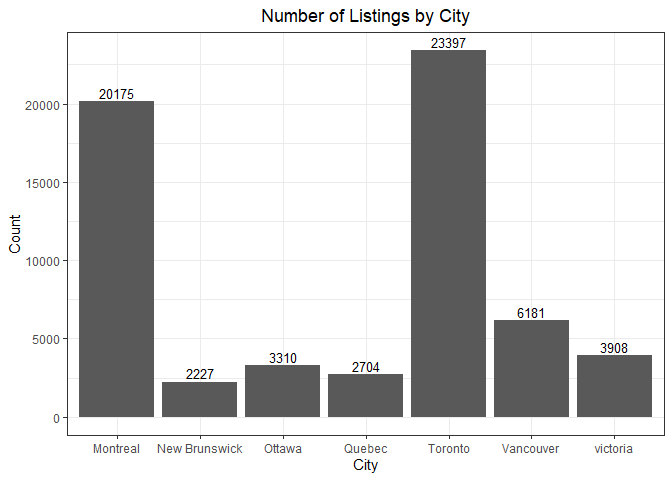
\includegraphics{../Images/Number_of_listings.png}

\hypertarget{how-many-airbnb-superhosts-are-there-in-different-canadian-cities}{%
\subsubsection{2. How many Airbnb superhosts are there in different
Canadian
cities?}\label{how-many-airbnb-superhosts-are-there-in-different-canadian-cities}}

The proportional bar chart below shows the percentage of superhosts in
different cities. From the plot, Victoria seems to have the largest
percentage of superhosts (48.0886850152905\%), while Montreal seems to
have the smallest percentage of superhosts (19.3784813837584\%).

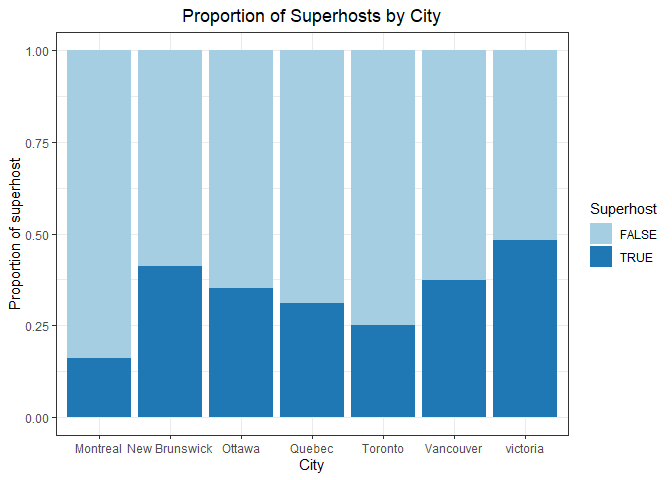
\includegraphics{../Images/Proportion_of_superhosts.png}

\hypertarget{is-there-a-relationship-between-the-number-of-accommodates-and-other-features-of-the-listing}{%
\subsubsection{3. Is there a relationship between the number of
accommodates and other features of the
listing?}\label{is-there-a-relationship-between-the-number-of-accommodates-and-other-features-of-the-listing}}

From the correllogram below, there is a strong relationship between the
number of accommodates and the number of beds in the unit. This may
cause a problem when performing linear regression analysis because some
predictors are collinear. To solve the collinearity problem, we may
decide to not use all of the variables (accommodates, bathrooms,
bedrooms, and beds) as predictors in the linear regression model.

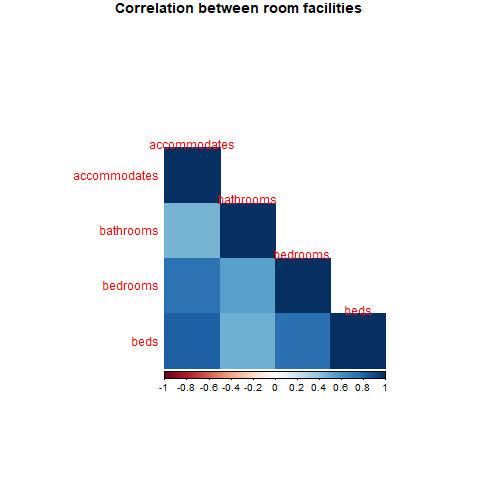
\includegraphics{../Images/Correlation_between_room_facilities.png}

\hypertarget{what-is-the-distribution-of-the-price-per-night-in-different-canadian-cities}{%
\subsubsection{4. What is the distribution of the price per night in
different Canadian
cities?}\label{what-is-the-distribution-of-the-price-per-night-in-different-canadian-cities}}

The side-by-side boxplots shows the price per night (after log10
transformation) distribution in different cities. From the plots, we can
see that there are some extremely high prices in the dataset. Further
analysis will be required to figure out the reason for the extreme
prices. Otherwise, we may need to consider them as outliers.

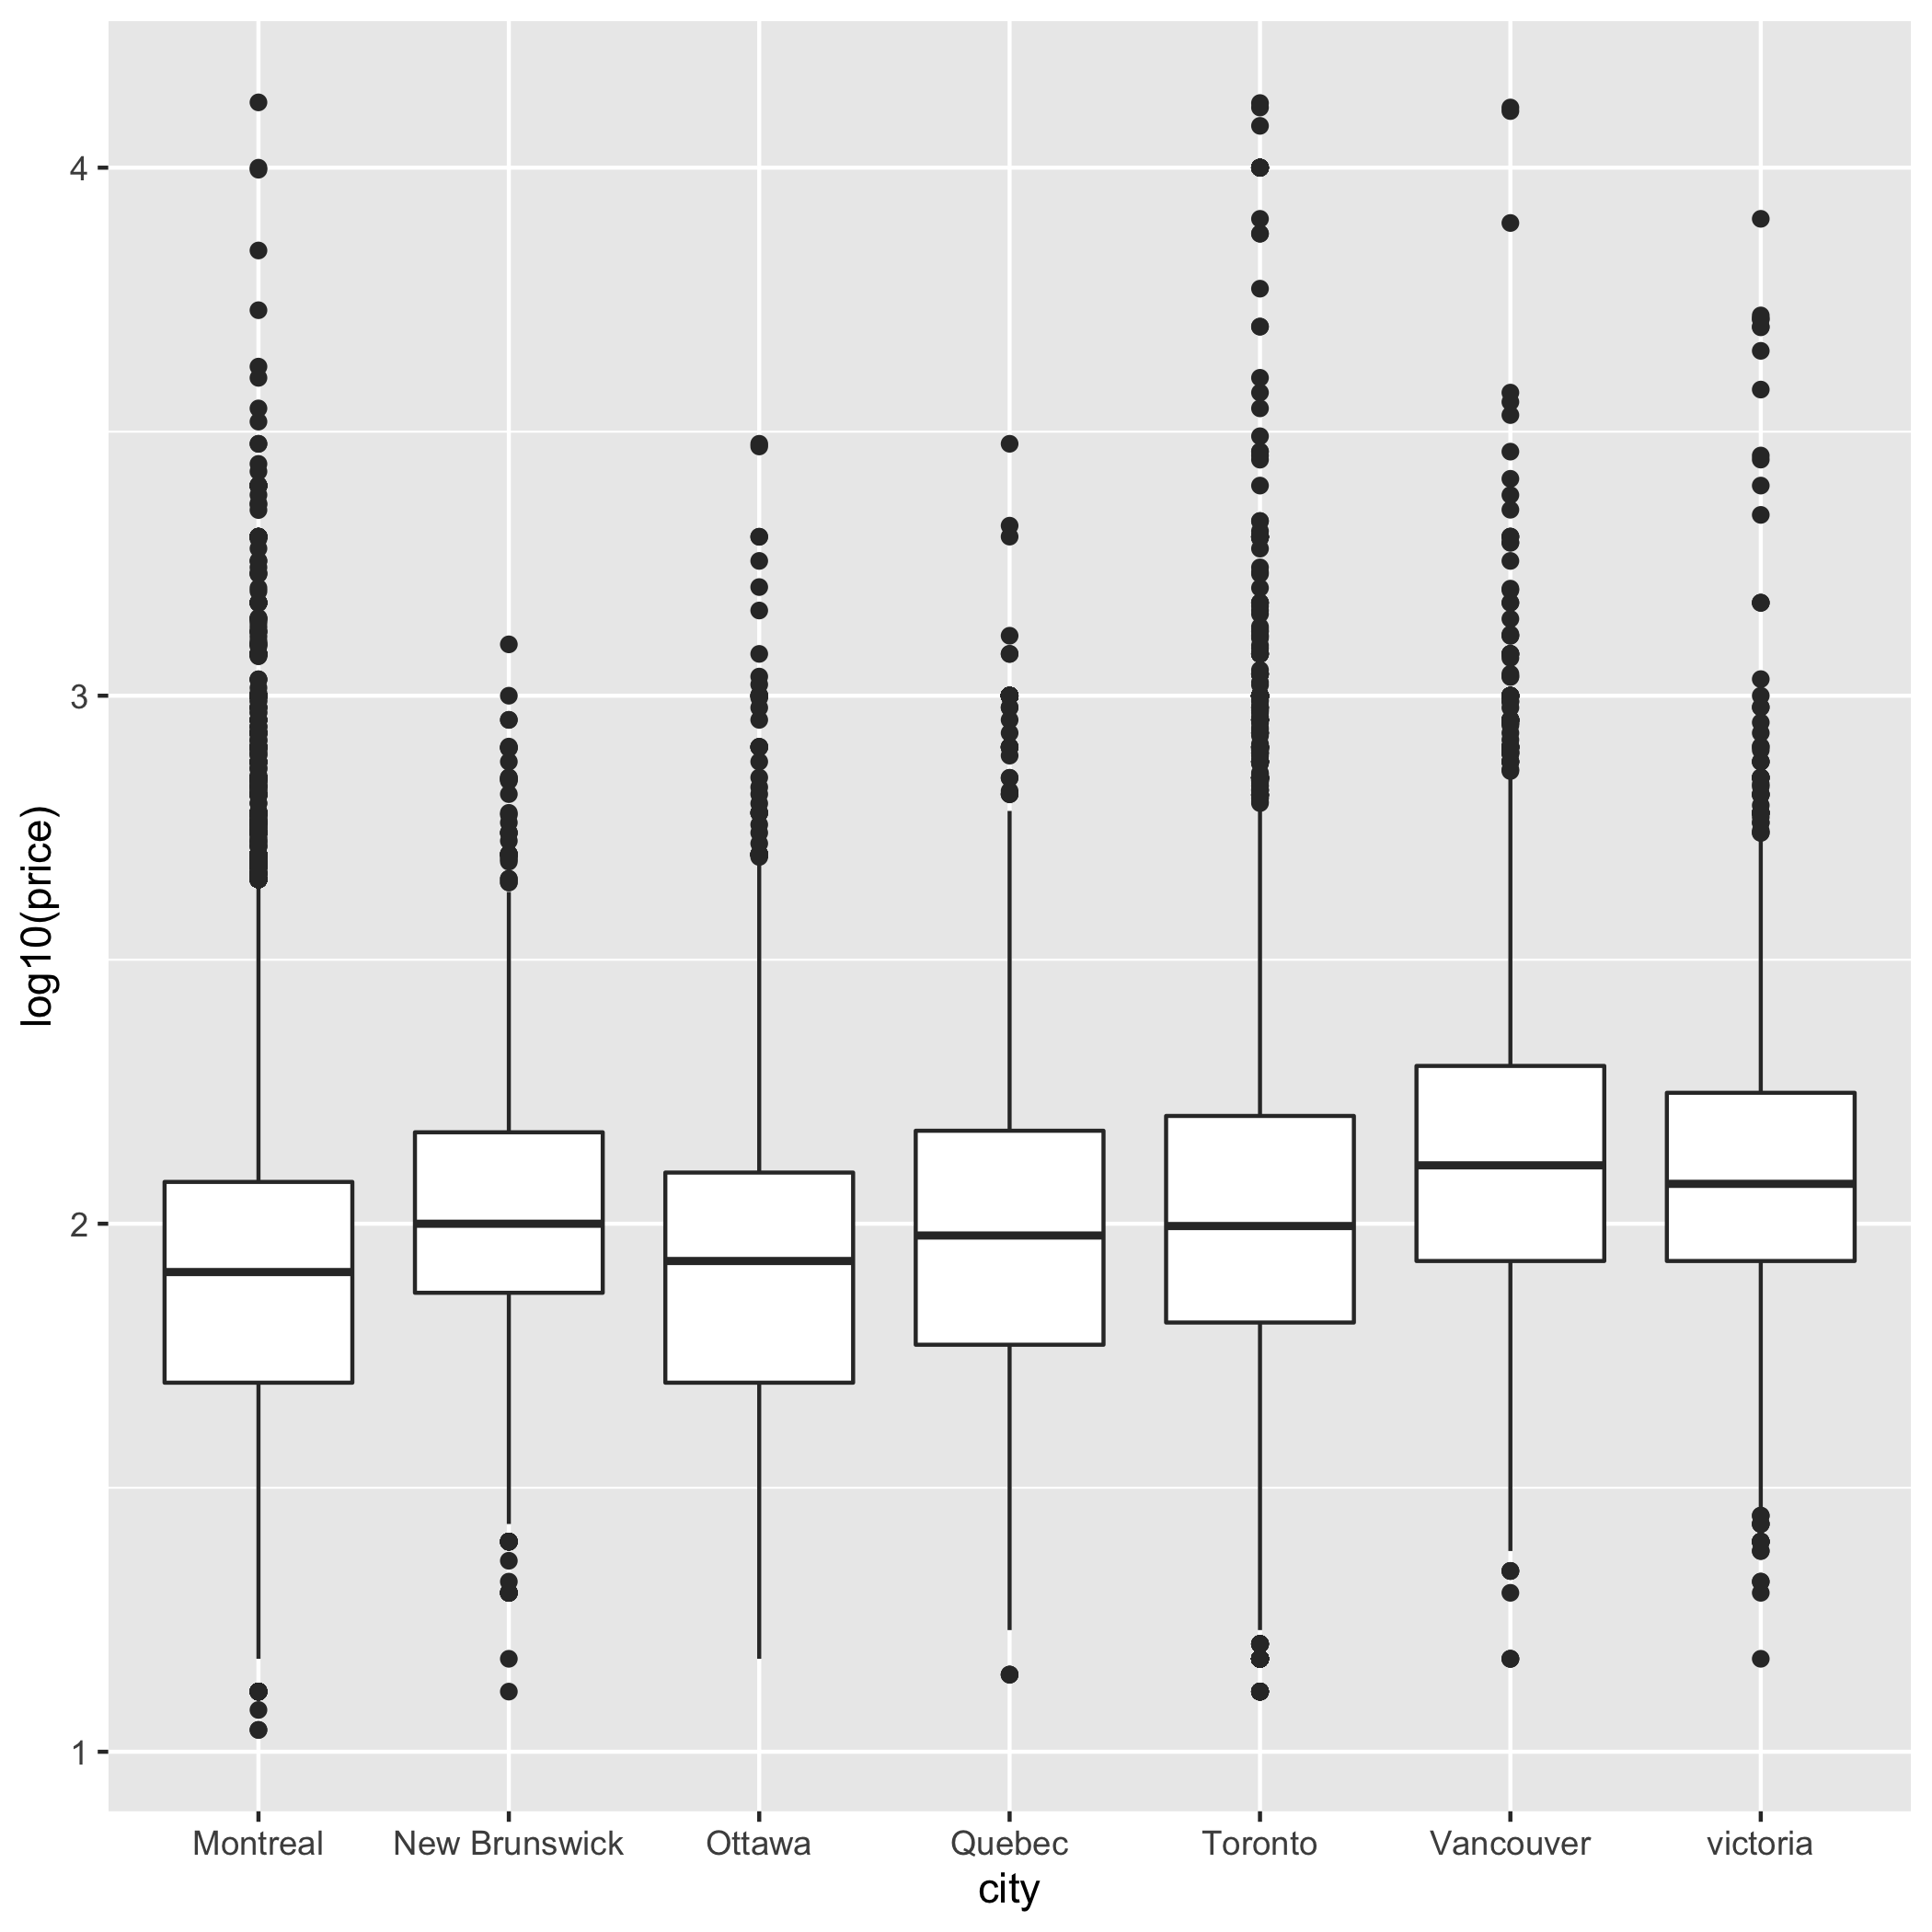
\includegraphics{../Images/Boxplot_of_price.png}

\hypertarget{analysis-methods}{%
\subsection{Analysis Methods}\label{analysis-methods}}

To identify which variables are most likely influencing the price of
Canadian Airbnb listings, we developed an analysis protocol which
consists of 3 steps.\\
1) Remove all the outliers 2) Fit a linear regression model 3) Perform
model diagnostics to check the assumptions and the model performance

\hypertarget{step-1-remove-outliers}{%
\subsubsection{Step 1: Remove Outliers}\label{step-1-remove-outliers}}

We classified an observation as an outlier if it fell below
\texttt{Q1-1.5*IQR} or above \texttt{Q3+1.5*IQR}, where Q1 and Q3
represents the first and third quantile of all the observations in the
corresponding city; IQR means interquartile range (\texttt{Q3-Q1}).

\hypertarget{step-2-fit-a-linear-regression-model}{%
\subsubsection{Step 2: Fit a linear regression
model}\label{step-2-fit-a-linear-regression-model}}

We built a full model for \texttt{price} by including all the potential
predictors mentioned in the Data Description section. Next, we performed
variable selection. Since the \texttt{property\ type} variable had too
many levels (44 levels), it was not appropriate to include this in the
linear regression model. In addition, the \texttt{bed} variable was
removed because it was highly correlated with \texttt{accommodates},
\texttt{bathrooms}, and \texttt{bedrooms}.

\hypertarget{step-3-model-diagnostics}{%
\subsubsection{Step 3: Model
Diagnostics}\label{step-3-model-diagnostics}}

Four plots were produced for model checking. The first plot is a
residual vs.~fitted values plot. It is useful for checking the
assumption of linearity. The second plot is a QQ plot and this is used
to check the normality assumption of the residuals. The third plot is a
scale-location plot and this is useful for checking the assumption of
homoscedasticity. The fourth plot is a Cook's distance plot and this
shows the measure of the influence of each observation on the regression
coefficients.

\hypertarget{results}{%
\subsection{Results}\label{results}}

Let's look at the results of the linear regression model.

\begin{Shaded}
\begin{Highlighting}[]
\NormalTok{lm <-}\StringTok{ }\KeywordTok{readRDS}\NormalTok{(here}\OperatorTok{::}\KeywordTok{here}\NormalTok{(}\StringTok{"RDS"}\NormalTok{,}\StringTok{"step_lm.RDS"}\NormalTok{))}
\NormalTok{knitr}\OperatorTok{::}\KeywordTok{kable}\NormalTok{(}\KeywordTok{tidy}\NormalTok{(lm))}
\end{Highlighting}
\end{Shaded}

\begin{longtable}[]{@{}lrrrr@{}}
\toprule
term & estimate & std.error & statistic & p.value\tabularnewline
\midrule
\endhead
(Intercept) & 49.389185 & 0.6988047 & 70.676663 &
0.0000000\tabularnewline
host\_is\_superhostTRUE & 2.603737 & 0.4339549 & 6.000017 &
0.0000000\tabularnewline
cityNew Brunswick & 14.695022 & 1.0447213 & 14.065973 &
0.0000000\tabularnewline
cityOttawa & 8.380514 & 0.9020077 & 9.290956 & 0.0000000\tabularnewline
cityQuebec & 11.040100 & 0.9611550 & 11.486284 &
0.0000000\tabularnewline
cityToronto & 32.873827 & 0.4621202 & 71.136957 &
0.0000000\tabularnewline
cityVancouver & 50.329410 & 0.7032114 & 71.570815 &
0.0000000\tabularnewline
cityvictoria & 33.765144 & 0.8410008 & 40.148764 &
0.0000000\tabularnewline
room\_typeHotel room & 8.141642 & 2.8297850 & 2.877124 &
0.0040146\tabularnewline
room\_typePrivate room & -45.298859 & 0.4728658 & -95.796437 &
0.0000000\tabularnewline
room\_typeShared room & -64.408283 & 1.7562995 & -36.672722 &
0.0000000\tabularnewline
accommodates & 6.997359 & 0.1526387 & 45.842622 &
0.0000000\tabularnewline
bathrooms & 10.315506 & 0.4515773 & 22.843279 & 0.0000000\tabularnewline
bedrooms & 8.956279 & 0.3183921 & 28.129718 & 0.0000000\tabularnewline
cancellation\_policymoderate & -2.397571 & 0.4991631 & -4.803182 &
0.0000016\tabularnewline
cancellation\_policystrict & 4.076218 & 0.4789944 & 8.509951 &
0.0000000\tabularnewline
cancellation\_policysuper\_strict & 33.610818 & 3.6772103 & 9.140303 &
0.0000000\tabularnewline
\bottomrule
\end{longtable}

\begin{itemize}
\tightlist
\item
  The coefficient of \texttt{superhost} is positive and this means that
  if the host is a superhost, the Airbnb price will be higher than if a
  host was not a superhost.
\item
  Montreal is a baseline \texttt{city} meaning that the Airbnb price in
  Montreal is the lowest compared to the other cities. In contrast, the
  Airbnb price in Vancouver is the highest. On average, the price in
  Vancouver is \$50 higher than the price in Montreal using our model.\\
\item
  For the \texttt{room\ type} variable, apartment is the baseline. If
  the room type is a hotel room, the price is higher. However, if the
  room type is a private room, the price is lower. Finally, if the room
  type is a shared room, the price is even lower at about \$64.
\item
  The coefficient of \texttt{accommodates} is 7 which means that for
  each extra accommodate, the Airbnb price increases by \$7 on average.
\item
  The coefficient of \texttt{bathroom} is 10 which means that for each
  extra bathroom, the Airbnb price increases by \$10 on average.
\item
  The coefficient of \texttt{bedroom} is 9 which means that for each
  extra bathroom, the Airbnb price increases by \$9 on average.
\item
  For the \texttt{cancellation\ policy} variable, flexible cancellation
  is the baseline. Airbnb listings with a moderate cancellation policy
  has a lower price while the Airbnb listings with a strict or super
  strict cancellation policy has a higher price.
\end{itemize}

Next, let's take a look at the model diagnostics:

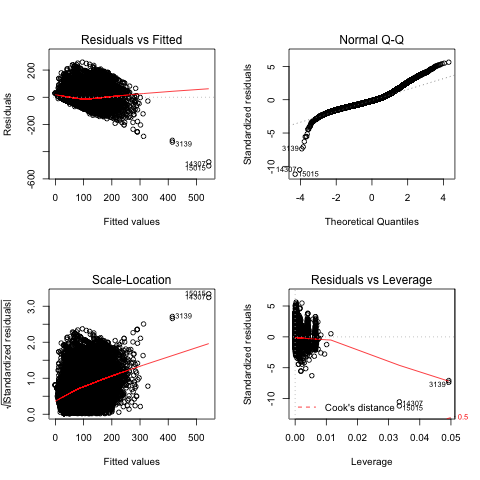
\includegraphics{../Images/Model_Diagnostics.png}

There is an increasing trend in the scale-location plot, so the
assumption of homoscedasticity may not hold. From the Cook's distance
plot, there are several influential points (far right), which may
require us to remove in the future analysis.

\hypertarget{conclusionsdiscussion}{%
\subsection{Conclusions/Discussion}\label{conclusionsdiscussion}}

In conclusion, there appears to be certain variables that have a
significant effect on Canadian Airbnb listings. Variables such as
superhost, city, room type, number of accommodates, number of bathrooms,
number of bedrooms, and cancellation policy. However, the model does not
seem to fit very well based on the model diagnostics. A possible reason
is that there are too many categorical variables included in the linear
regression model, which is one of the limitations for this study. For
future analysis, we will consider removing the influential points and
performing ANOVA instead of linear regression.

\hypertarget{references}{%
\subsection{References}\label{references}}

Statistics Canada. (2020, February 21). Travel between Canada and other
countries, December 2019. Retrieved from
\url{https://www150.statcan.gc.ca/n1/daily-quotidien/200221/dq200221b-eng.htm?indid=3635-2\&indgeo=0}

\end{document}
